\documentclass[11pt]{article}

\usepackage[margin=1in]{geometry}
\usepackage{amsmath}
\usepackage{booktabs}
\usepackage{graphicx}
\usepackage{microtype}
\usepackage{tabularx}
\usepackage[numbers,sort&compress]{natbib}
\usepackage{xcolor}
\usepackage[hidelinks]{hyperref}
\usepackage{url}

\newcommand{\method}{Matched Position--Supervision Factorial Study}
\newcommand{\pending}[1]{\textcolor{red}{[PENDING: #1]}}
% Generated from audited seed-level result JSON; do not hand-edit.
\newcommand{\ExploratoryRuleAnswerMin}{97.3\%}
\newcommand{\ExploratoryRuleAnswerMax}{100.0\%}
\newcommand{\ExploratoryPairedAnswerWorst}{87.3\%}
\newcommand{\ExploratoryPairedAnswerGap}{12.7\%}
\newcommand{\ExploratoryIndependentEvidenceWorst}{99.7\%}
\newcommand{\ExploratoryIndependentEvidenceGap}{0.3\%}
\newcommand{\GeneratedMainRows}{%
Mistral-7B-v0.3 & -- & -- & 63.3 & 39.0 & 60.7 & 53.4 \\
Mistral-7B-v0.3 & Independent & Answer & 95.4 & 89.9 & 10.1 & 0.0 \\
Mistral-7B-v0.3 & Independent & Evidence ID & 92.5 & 84.2 & 15.6 & 0.0 \\
Mistral-7B-v0.3 & Independent & Exact evidence & 77.1 & 69.6 & 17.9 & 76.7 \\
Mistral-7B-v0.3 & Paired & Answer & 75.8 & 63.7 & 26.1 & 0.0 \\
Mistral-7B-v0.3 & Paired & Evidence ID & 94.4 & 88.5 & 11.5 & 0.0 \\
Mistral-7B-v0.3 & Paired & Exact evidence & 99.4 & 96.7 & 3.3 & 82.9 \\
\addlinespace
Qwen2.5-7B & -- & -- & 69.2 & 41.5 & 51.2 & 68.3 \\
Qwen2.5-7B & Independent & Answer & 98.0 & 92.9 & 7.1 & 0.0 \\
Qwen2.5-7B & Independent & Evidence ID & 99.7 & 98.7 & 1.3 & 0.0 \\
Qwen2.5-7B & Independent & Exact evidence & 99.6 & 97.9 & 2.1 & 99.8 \\
Qwen2.5-7B & Paired & Answer & 97.2 & 90.8 & 9.2 & 0.0 \\
Qwen2.5-7B & Paired & Evidence ID & 99.7 & 98.2 & 1.8 & 0.0 \\
Qwen2.5-7B & Paired & Exact evidence & 99.5 & 97.6 & 2.4 & 99.8 \\
}
\newcommand{\GeneratedNoLiMaRows}{%
Mistral-7B-v0.3 & -- & -- & 12.9 & 4.8 & 32.6 & 16.7 \\
Mistral-7B-v0.3 & Independent & Answer & 9.8 & 2.3 & 32.1 & 0.0 \\
Mistral-7B-v0.3 & Independent & Evidence ID & 18.4 & 7.4 & 34.8 & 0.0 \\
Mistral-7B-v0.3 & Independent & Exact evidence & 16.7 & 4.0 & 50.6 & 10.5 \\
Mistral-7B-v0.3 & Paired & Answer & 4.0 & 0.0 & 21.0 & 0.0 \\
Mistral-7B-v0.3 & Paired & Evidence ID & 17.9 & 7.8 & 35.7 & 0.0 \\
Mistral-7B-v0.3 & Paired & Exact evidence & 13.8 & 4.6 & 34.1 & 16.2 \\
\addlinespace
Qwen2.5-7B & -- & -- & 17.7 & 7.0 & 40.4 & 13.8 \\
Qwen2.5-7B & Independent & Answer & 13.0 & 1.7 & 40.4 & 0.0 \\
Qwen2.5-7B & Independent & Evidence ID & 13.3 & 2.6 & 36.2 & 0.0 \\
Qwen2.5-7B & Independent & Exact evidence & 15.5 & 3.2 & 44.2 & 11.0 \\
Qwen2.5-7B & Paired & Answer & 15.7 & 2.3 & 51.9 & 0.0 \\
Qwen2.5-7B & Paired & Evidence ID & 13.7 & 3.8 & 37.2 & 0.0 \\
Qwen2.5-7B & Paired & Exact evidence & 15.5 & 5.6 & 42.2 & 13.9 \\
}
\newcommand{\GeneratedLongBenchRows}{%
Mistral-7B-v0.3 & -- & -- & 46.4 & 28.3 & 23.4 & 32.7 \\
Mistral-7B-v0.3 & Independent & Answer & 47.8 & 31.0 & 20.6 & 33.1 \\
Mistral-7B-v0.3 & Independent & Evidence ID & 52.1 & 37.9 & 24.8 & 38.3 \\
Mistral-7B-v0.3 & Independent & Exact evidence & 29.7 & 23.3 & 14.9 & 22.6 \\
Mistral-7B-v0.3 & Paired & Answer & 35.6 & 25.0 & 15.1 & 25.2 \\
Mistral-7B-v0.3 & Paired & Evidence ID & 50.8 & 36.3 & 22.4 & 36.5 \\
Mistral-7B-v0.3 & Paired & Exact evidence & 27.4 & 24.7 & 14.3 & 22.1 \\
\addlinespace
Qwen2.5-7B & -- & -- & 58.3 & 43.3 & 29.5 & 43.7 \\
Qwen2.5-7B & Independent & Answer & 53.2 & 44.3 & 23.1 & 40.2 \\
Qwen2.5-7B & Independent & Evidence ID & 52.0 & 42.2 & 22.6 & 39.0 \\
Qwen2.5-7B & Independent & Exact evidence & 55.8 & 44.7 & 27.5 & 42.7 \\
Qwen2.5-7B & Paired & Answer & 55.5 & 45.7 & 27.1 & 42.8 \\
Qwen2.5-7B & Paired & Evidence ID & 55.2 & 42.2 & 26.5 & 41.3 \\
Qwen2.5-7B & Paired & Exact evidence & 55.5 & 43.4 & 28.0 & 42.3 \\
}
\newcommand{\GeneratedFactorialContrastRows}{%
Mistral-7B-v0.3 & Paired $-$ independent & +1.7 [-78.7, +82.2] & -0.9 [-55.6, +53.8] & -0.5 [-5.4, +4.5] & -8.9 [-27.3, +9.4] & -3.4 [-17.8, +11.1] \\
Mistral-7B-v0.3 & Evidence ID $-$ answer & +9.6 [-32.3, +51.5] & -4.5 [-27.4, +18.3] & +6.4 [+0.9, +12.0] & +8.7 [-4.7, +22.1] & +8.2 [-10.1, +26.6] \\
Mistral-7B-v0.3 & Exact evidence $-$ answer & +6.4 [-66.2, +78.9] & -7.5 [-42.7, +27.8] & +3.1 [-2.9, +9.1] & +15.8 [-9.1, +40.7] & -6.8 [-15.5, +2.0] \\
Mistral-7B-v0.3 & Pairing $\times$ exact-vs-answer & +53.3 [+8.7, +97.9] & -30.6 [-35.4, -25.8] & +3.0 [-1.6, +7.6] & -5.4 [-58.6, +47.7] & +7.4 [-34.0, +48.7] \\
\addlinespace
Qwen2.5-7B & Paired $-$ independent & -1.0 [-5.4, +3.4] & +1.0 [-3.4, +5.4] & +1.4 [-1.7, +4.5] & +3.5 [-16.4, +23.4] & +1.5 [-2.5, +5.5] \\
Qwen2.5-7B & Evidence ID $-$ answer & +6.5 [-6.5, +19.6] & -6.5 [-19.6, +6.5] & +1.2 [+0.5, +1.9] & -9.4 [-17.9, -1.0] & -1.4 [-7.9, +5.2] \\
Qwen2.5-7B & Exact evidence $-$ answer & +5.9 [-6.5, +18.3] & -5.9 [-18.3, +6.5] & +2.3 [+1.6, +3.0] & -2.9 [-27.2, +21.4] & +1.0 [+0.2, +1.8] \\
Qwen2.5-7B & Pairing $\times$ exact-vs-answer & +1.8 [-3.4, +7.0] & -1.8 [-7.0, +3.4] & +1.7 [-2.6, +6.1] & -13.5 [-54.7, +27.7] & -3.0 [-10.1, +4.1] \\
}
\newcommand{\GeneratedRegressionRows}{%
Qwen2.5-7B & -- & -- & 67.0 & -- & 72.5 & -- \\
Qwen2.5-7B & Independent & Answer & 66.7 & Pass & 70.2 & Fail \\
Qwen2.5-7B & Independent & Evidence ID & 66.6 & Pass & 69.5 & Fail \\
Qwen2.5-7B & Independent & Exact evidence & 67.0 & Pass & 71.5 & Fail \\
Qwen2.5-7B & Paired & Answer & 66.8 & Pass & 69.7 & Fail \\
Qwen2.5-7B & Paired & Evidence ID & 66.3 & Pass & 70.4 & Fail \\
Qwen2.5-7B & Paired & Exact evidence & 66.4 & Pass & 71.3 & Fail \\
\addlinespace
Mistral-7B-v0.3 & -- & -- & 54.2 & -- & 43.1 & -- \\
Mistral-7B-v0.3 & Independent & Answer & 52.6 & Fail & 40.1 & Fail \\
Mistral-7B-v0.3 & Independent & Evidence ID & 54.9 & Pass & 42.9 & Fail \\
Mistral-7B-v0.3 & Independent & Exact evidence & 53.6 & Pass & 45.1 & Pass \\
Mistral-7B-v0.3 & Paired & Answer & 34.3 & Fail & 21.3 & Fail \\
Mistral-7B-v0.3 & Paired & Evidence ID & 53.2 & Pass & 39.2 & Fail \\
Mistral-7B-v0.3 & Paired & Exact evidence & 53.8 & Pass & 40.7 & Fail \\
}
\newcommand{\GeneratedMechanismRows}{%
Qwen2.5-7B & -- & -- & 17.7 & 6.0 & 0.7 & 100.0 \\
Qwen2.5-7B & Independent & Answer & 10.8 & 0.0 & 0.7 & 98.0 \\
Qwen2.5-7B & Independent & Exact evidence & 18.2 & 34.7 & 5.3 & 100.0 \\
Qwen2.5-7B & Paired & Answer & 16.1 & 0.0 & 2.0 & 100.0 \\
Qwen2.5-7B & Paired & Exact evidence & 15.6 & 35.8 & 0.7 & 99.3 \\
\addlinespace
Mistral-7B-v0.3 & -- & -- & 12.9 & 34.8 & 54.7 & 100.0 \\
Mistral-7B-v0.3 & Independent & Answer & 14.3 & 0.0 & 96.7 & 72.7 \\
Mistral-7B-v0.3 & Independent & Exact evidence & 24.2 & 6.2 & 84.7 & 98.7 \\
Mistral-7B-v0.3 & Paired & Answer & 0.2 & 0.0 & 10.0 & 88.0 \\
Mistral-7B-v0.3 & Paired & Exact evidence & 16.8 & 13.9 & 84.0 & 89.3 \\
}


\title{Pairing Positions or Supervising Evidence?\\
A Matched Factorial Study of Long-Context Position Robustness}
\author{\pending{author names, order, affiliations, and contact email}}
\date{}

\begin{document}
\maketitle

\begin{abstract}
Long-context language models often answer less reliably when relevant evidence moves within an otherwise unchanged input. Existing training work changes several factors at once, making it unclear whether improvements come from repeated facts, balanced locations, explicit cross-position pairing, or richer evidence supervision. We introduce a compute-matched $2\times3$ factorial study that independently varies position construction (independent versus paired) and supervision (answer, evidence ID, or exact evidence quote). Every strict contrast holds facts, exposure counts, filler realizations, sequence counts, position histograms, and input-token budgets fixed. We evaluate answer correctness, evidence verifiability, worst-position accuracy, and position gap on seven-location controlled tests; semantic retrieval without literal overlap using NoLiMa; and natural multi-document transfer using LongBench. We use three fixed training/data seeds per model family and disclose a realized-sampler audit that demoted an initially incomplete Qwen pairing implementation to exploratory status before rerunning block-complete adapters. Across Qwen2.5-7B and Mistral-7B families, \pending{insert strict block-96 result and uncertainty}. Our results distinguish distribution-specific repair from robust long-context utilization and provide an auditable protocol for attributing gains to training position structure and supervision content.
\end{abstract}

\section{Introduction}

Supporting a long input is not equivalent to using every part of it reliably. Position-controlled evaluations show that moving the same relevant passage can change model behavior, often yielding stronger performance at context boundaries than in the middle \citep{liu2024lost}. The curve is not universal: its shape depends on relative input length, task structure, and retrieval difficulty. Moreover, literal needle tests can overestimate usable context because a model can exploit lexical matches rather than recover a latent association \citep{modarressi2025nolima}.

Training with information-intensive, shuffled, or evidence-grounded long-context examples can flatten position curves \citep{an2024film,he2024never,yuan2026longcrafter}. Yet prior interventions commonly change data volume, task diversity, difficulty, evidence format, and position distribution together. Consequently, an improvement cannot be cleanly attributed to seeing facts at more locations, seeing the \emph{same} fact across locations, or receiving a target that explicitly identifies supporting evidence.

We isolate these factors with a matched factorial design. The position factor contrasts independent location sampling with explicit position-equivalent pairing. The supervision factor contrasts answer-only targets, answer plus evidence-document IDs, and answer plus exact source quotes. All six cells use identical facts and filler views under matched sequence and token budgets. This design asks two focused questions: (i) does explicit cross-position pairing improve the weakest location beyond position-balanced independent sampling, and (ii) does increasingly verifiable supervision change answer robustness or merely output format?

Our contributions are:
\begin{itemize}
    \item a matched $2\times3$ causal attribution design for position construction and supervision granularity;
    \item a position-equivalent evaluation protocol reporting weakest-position accuracy, gap, evidence validity, and paired uncertainty rather than only mean accuracy;
    \item complementary distribution-shift tests: controlled NoLiMa semantic retrieval and natural LongBench multi-document QA;
    \item a reproducibility package containing data-generation audits, model and environment hashes, per-step training traces, license-safe per-sample audit records, and saved bootstrap indices.
\end{itemize}

\section{Related Work}

\paragraph{Position-dependent context use.}
Lost in the Middle established controlled multi-document QA and key--value retrieval tests in which the location of relevant content changes while content remains fixed \citep{liu2024lost}. RULER broadened synthetic long-context evaluation across retrieval, tracking, aggregation, and question answering \citep{hsieh2024ruler}. LongBench complements controlled tests with 21 natural and synthetic tasks, but does not by itself identify a causal position effect \citep{bai2024longbench}. NoLiMa removes direct lexical matches between question and evidence and shows that many models degrade well before their advertised context limit \citep{modarressi2025nolima}. Veseli et al. normalize input length by each model's maximum context and show that the familiar U-shape is strongest at relative lengths up to one half; nearer the limit, primacy weakens while recency remains, so a missing U-shape need not imply position invariance \citep{veseli2025shift}. CRE independently audits the reasoning-benchmark gap by jointly varying target position, filler content, and context length on GSM8K and ARC-Challenge; its model- and filler-dependent failures reinforce the need to report position-conditioned rather than aggregate scores \citep{zhang2026positional}. We combine strict within-group position control with natural transfer instead of treating either as sufficient alone.

These evaluation studies establish the phenomenon but do not identify which training-data property repairs it. In particular, CRE changes evaluation context while leaving each evaluated model fixed, and Veseli et al. characterize curve shape across relative lengths. Our contribution is orthogonal: we randomize training position construction and target supervision under identity-, exposure-, sequence-, and prompt-token-matched budgets, then test whether any resulting repair transfers to their harder semantic and natural regimes. We therefore make no claim that the controlled benchmark or position metric itself is new.

Concurrent small-transformer work gives a complementary identifiability warning: when position and repetition cues are exactly coextensive in a synthetic document distribution, all runs can attain essentially perfect held-in accuracy while the intervention-based rule readout varies sharply across seeds \citep{liao2026shortcut}. That study concerns mechanism selection during synthetic pretraining rather than long-context adaptation, so it is not an intervention baseline for our 7B models. It nevertheless motivates separating co-varying training factors and treating independent training seeds as the unit of replication instead of inferring a mechanism from aggregate accuracy alone.

\paragraph{Inference-time and positional-encoding interventions.}
Found in the Middle estimates a content-independent positional attention baseline by moving a fixed context, then calibrates document attention for RAG; it improves NaturalQuestions and SynthWiki but requires an additional $O(K)$ forward passes for $K$ document positions \citep{hsieh2024found}. LPES instead searches a smooth layer-specific RoPE-scaling curve on 200 examples, leaves model weights unchanged, and uses a single forward pass after the search \citep{lv2026lpes}. Both intervene on inference or positional encoding. Our study asks a different training-time attribution question: under fixed facts, exposures, sequences, and prompt-token budgets, does explicit identity-preserving cross-position pairing or richer completion supervision produce transferable robustness? We therefore do not claim these approaches are interchangeable, and we reserve architectural or inference-time combinations for future work.

\paragraph{Training interventions.}
Position-Agnostic Multi-step QA trains question repetition, evidence-index prediction, and answer generation on shuffled documents \citep{he2024never}. IN2 constructs information-intensive examples with critical spans distributed throughout long contexts \citep{an2024film}. LongCrafter uses a task taxonomy, evidence-constraint graphs, and cited responses to produce difficult and faithful long-context supervision \citep{yuan2026longcrafter}. These studies establish that data design matters, but do not fully separate explicit cross-position pairing from the information content of the target at equal budgets. Our evidence-ID cell is an intermediate treatment between answer-only and exact quotation, allowing a graded test of localization supervision.

Pos2Distill is the closest same-example cross-position precedent: for retrieval it transfers the output distribution at an advantageous evidence position to a disadvantaged one with a KL objective, while its reasoning variant distills a high-quality chain of thought across positions \citep{wang2025pos2distill}. It therefore jointly introduces position pairing, an asymmetric teacher--student direction, and a specialized distillation target. Our study does not claim that cross-position identity reuse is new; instead, its factorial controls test whether identity-preserving pairing itself contributes beyond a matched independent position histogram, and whether any effect depends on answer, evidence-ID, or exact-quote supervision without a teacher model or KL loss.

RoPE-Perturbed Self-Distillation forms a standard and an index-shifted view of the same long sequence, then adds a stop-gradient reverse-KL consistency loss; it reports two-family gains on RULER and HELMET, length extrapolation, LongBench-v2 transfer, short-task retention, and a matched-wall-time control \citep{li2026shuffle}. Randomized YaRN instead assigns ordered random YaRN indices drawn from an expanding curriculum during short-context LoRA and evaluates reasoning beyond the training length on BABILong and MRCR in two 7B families \citep{mehta2026randomized}. These are important positive intervention baselines, but both change positional encoding exposure and the optimization objective. We hold RoPE, inference, and completion-only optimization fixed to isolate data-identity pairing and supervision content; our negative or null transfer results therefore do not contradict gains from stronger position-encoding regularizers.

FOCUSFT addresses a different training mechanism: an inner fast-weight loop forms a context-conditioned parametric memory and an outer SFT loop learns from that sharpened representation, with bidirectional attention over context tokens in both loops \citep{pei2026focusft}. It reports strong BABILong and RULER gains with unchanged inference cost, but uses one Qwen2.5-7B family and incurs 1.71$\times$ training wall time. Our fixed completion-only QLoRA objective leaves attention masks and optimization structure unchanged, making the present question narrower: which matched data construction and target content, if any, improve robustness?

EXACT isolates a complementary objective-level intervention: with the packed continued-pretraining stream, token budget, optimizer, and subsequent QA tuning fixed, it upweights rare targets whose same-document effective left context is long \citep{zhu2026exact}. Its controls distinguish effective-context weighting from random weighting and absolute packed-position weighting, but it does not compare whether the same underlying fact is explicitly paired across positions or whether answer, identifier, and exact-quote targets differ under matched completion-only SFT. Our factorial analysis therefore addresses a data-identity and target-content question rather than a causal-LM loss-allocation question.

\section{Experimental Design}

\subsection{Matched factorial treatments}

Let $f$ denote an underlying fact set, $v$ a fixed filler realization, and $p\in P$ one of seven relative positions $P=\{0,.1,.25,.5,.75,.9,1\}$. A position-equivalent group $G(f,v)=\{x(f,v,p):p\in P\}$ changes only evidence placement. Training treatments cross:
\begin{align*}
\text{pairing} &\in \{\text{independent},\text{paired}\},\\
\text{supervision} &\in \{\text{answer},\text{evidence-ID},\text{exact-evidence}\}.
\end{align*}
Independent construction draws locations separately while matching the aggregate position histogram. Paired construction samples multiple members of the same $G(f,v)$ together. The supervision target is respectively an answer string; an answer with the supporting document identifiers; or an answer with identifiers and minimal verbatim supporting spans.

Across all six cells we hold the underlying fact bank, fact exposure counts, filler replicas, sequence count, and prompt-token budget fixed. Target lengths differ by design, so absolute completion loss is used only as a within-run health diagnostic, not as a treatment outcome.

\subsection{Data provenance and teacher independence}

Controlled facts, questions, fillers, answers, evidence identifiers, and minimal quotes are generated locally from deterministic templates and exact verifiers. We do not use DeepSeek or another proprietary teacher to produce targets. This keeps target quality identical across factorial cells and avoids introducing an unmeasured teacher-style or position preference. Natural evaluations are prepared only from pinned public benchmark revisions; no evaluation answer is used for training. Dataset manifests record source revision, generation arguments, tokenizer/chat-template fingerprint, row counts, group structure, and SHA-256 values.

\subsection{Models and training}

We use Qwen2.5-7B-Instruct and Mistral-7B-Instruct-v0.3 as similarly sized but distinct model families. Each family uses three fixed training/data seeds and all six factorial cells. The strict primary design selects 24 complete fact blocks per seed, with four replicas per fact, and adapts each model with 4-bit QLoRA for exactly 96 optimizer steps: rank 16, $\alpha=32$, dropout 0.05, completion-only cross entropy, batch size one, and deterministic data seeds. The resulting 96-row datasets are balanced at 24 rows per position; independent construction exposes each selected fact four times at one assigned position, while paired construction exposes it once at each of four positions. Fact/replica identities, task and length counts, and prompt-token totals are exactly matched across the pairing contrast. The 96-step budget is a design consequence---one complete pass over the materialized blocks---rather than a checkpoint selected by test performance.

\paragraph{Realized-subset correction.}
Our original frozen implementation used 1,024-row matched candidate datasets and a 100-step random sampler. After Qwen NoLiMa and part of LongBench had run, but before controlled confirmation or any Mistral training, we reconstructed the exact sampler order. Although the six cells retained identical ordered fact/replica identities and equal prompt-token totals, only 11--15 facts per seed received repeated cross-position exposure, no fact received all four paired positions, and the realized position histograms differed. We therefore treat every original fixed-100 result as a partial-dose exploratory sensitivity analysis, materialize the strict 96-row blocks above, and rerun all primary evaluations from new adapters. This correction was triggered by lineage rather than scores, but it is post hoc for Qwen and prospective only for Mistral; we report that distinction rather than relabeling the Qwen rerun as blindly preregistered.

Chat rendering is audited before model-specific tokenization. Qwen uses its native system--user--assistant protocol. Mistral-v0.3's native inference prompt retains the system instruction, but its full training render drops that turn and is therefore not prefix-safe for completion-only masking. For Mistral only, we freeze a deterministic compatibility protocol that merges the leading system text into the first user turn, separated by two newlines, before applying the native template in both training and inference. A sentinel audit verifies role preservation and exact token-prefix equality; the selected protocol, template and render hashes, tokenizer fingerprint, and model revision are recorded before any family-specific data are generated.

\subsection{Evaluation suites}

\paragraph{Controlled matched suite.}
The rule-based suite crosses retrieval and two-hop reasoning, nominal 8K and 32K lengths, neutral and answer-bearing interference, and seven evidence positions. Each model condition produces 4,200 predictions. Its role is internal validity: the exact same fact, question, and filler are compared within a position-equivalent group. Because chat templates tokenize differently, the long generator target is 32,768 tokens for Qwen and 32,512 for Mistral; the latter is still a 31.75K ``32K'' slice and differs by only 0.78\%. Before inference, all rendered prompts must satisfy prompt tokens plus the frozen 176-token output cap $\leq 32{,}768$. Exact realized lengths are retained in the released prompt-length audits rather than silently truncated.

\paragraph{NoLiMa semantic OOD.}
We derive a preregistered NoLiMa-Hard gate from the official data \citep{modarressi2025nolima}: 10 hard cases, five book haystacks, 1K/8K/32K lengths, and seven placements, totaling 1,050 prompts per model condition. Question, character, book slice, and length remain fixed within a group; only the official needle moves. No artificial evidence IDs are added. Exact quote output is scored, while evidence-ID accuracy is marked not applicable.

\paragraph{Natural multi-document transfer.}
We evaluate all 200 test examples from HotpotQA, 2WikiMultiHopQA, and MuSiQue in LongBench v1 \citep{bai2024longbench}. We use the official maximum English QA token-F1 over reference answers. These examples are natural but not position-controlled; accordingly they test task transfer and cannot establish a position effect.

\paragraph{Mechanism and regression checks.}
On NoLiMa-Hard, locate-only, oracle-long, and oracle-short variants distinguish evidence localization, evidence use under long interference, and answer generation with only gold evidence. Locate-only retains all 1,050 positioned prompts. Once evidence is moved into a tagged oracle block at the end, the seven source positions recover the same distractor context; we therefore deduplicate oracle-long and oracle-short to one input per 150 position-equivalent groups rather than treating redundant copies as observations. For each model family, we evaluate the base model and the four answer/exact-evidence corner treatments from the same frozen representative strict seed (20260825) and bootstrap the 10 underlying semantic cases as clusters. The Qwen representative is corrective and the Mistral representative prospective under the corrected protocol, so these mechanism results are diagnostic rather than multi-seed treatment estimates. Full-test MMLU option accuracy \citep{hendrycks2021mmlu} and official IFEval strict/loose prompt- and instruction-level accuracy \citep{zhou2023ifeval} check knowledge/reasoning and instruction-following retention with a preregistered two-percentage-point noninferiority margin. MMLU correctness uses a frozen format-robust extractor: it accepts the option from parsed JSON, a possibly truncated \texttt{answer} field, a bare option, or one unambiguous explicit answer phrase, in that order. Valid-JSON rate and output-cap hits remain separate generation diagnostics, so schema obedience cannot masquerade as knowledge loss.

\subsection{Metrics and statistics}
\label{sec:metrics}

For position-specific answer accuracy $A_p$, we report
\begin{align*}
A_{\mathrm{worst}} &= \min_{p\in P} A_p,\\
\Delta_{\mathrm{pos}} &= \max_{p\in P}A_p-\min_{p\in P}A_p,\\
\Delta_{\mathrm{mid}} &= (A_{0}+A_{1})/2-A_{.5}.
\end{align*}
We additionally report answer accuracy, valid JSON, evidence-ID accuracy when applicable, exact-quote accuracy when applicable, and whether every predicted quote occurs in the prompt.

The rule-controlled suite uses 5,000 position-equivalent-group bootstrap replicates stratified by task, filler, length, and evaluation mode. Both NoLiMa-Hard factorial and mechanism inference instead resample the 10 semantic cases as clusters, stratified by one-/two-hop task and keeping books, lengths, positions, modes, and model conditions paired inside each sampled case. The paper position figure combines NoLiMa's three task strata with their frozen 2/6/2 semantic-case weights within each seed before computing seed-level intervals; it does not give a two-case stratum the same weight as a six-case stratum. Natural transfer uses 5,000 question-level replicates paired across model conditions and stratified by task and word-length bin. We report treatment estimates and 95\% intervals for all preregistered main effects and interactions, with Holm correction within each metric family. Multi-seed inference treats seed as a training replicate rather than inflating it with within-seed examples.

We separately run a deterministic descriptive failure audit whose rule set was fixed after the exploratory Qwen diagnostics and before any strict block-96 outcomes. It exhaustively counts invalid JSON, answer errors, answer--quote disagreement, output-length caps, edge--middle reversals, answer changes across positions, Base-only or treatment-only successes, and treatment quote recoveries. Each rate retains its natural denominator: generated rows, eligible within-run groups, or matched Base--treatment comparisons; rates with different units are not pooled. Candidates are sorted by category, condition, group, and sample; at most five per category are retained for audit rather than chosen for narrative salience. The public catalog contains only structural fields, scored flags, and SHA-256 fingerprints---never prompts, targets, generated or parsed answers, quotes, raw identifiers, or absolute paths. Counts, rates, and examples are descriptive and do not alter the inferential family above.

\section{Results}

\subsection{Near-ceiling aggregate accuracy hides position failures}

The exploratory Qwen seed yields \ExploratoryRuleAnswerMin--\ExploratoryRuleAnswerMax\ aggregate answer accuracy across the six 100-step treatments. That range alone obscures large position differences: paired answer supervision has only \ExploratoryPairedAnswerWorst\ worst-position accuracy and a \ExploratoryPairedAnswerGap\ gap, whereas independent exact-evidence supervision reaches \ExploratoryIndependentEvidenceWorst\ worst-position accuracy with a \ExploratoryIndependentEvidenceGap\ gap. The frozen pilot therefore does not meet our formal all-cells saturation guard. We report it as evidence that aggregate accuracy can conceal positional failures and keep it outside strict-primary means; it cannot select a universally winning treatment.

\begin{table*}[t]
\centering
\scriptsize
\setlength{\tabcolsep}{3pt}
\caption{Primary strict block-complete factorial results. Treatment values are means across independently trained seeds, while Base is one fixed untrained model and is not duplicated as a training replicate. Qwen seeds are explicitly corrective and Mistral seeds prospective under this protocol. Uncertainty is defined in Section~\ref{sec:metrics}. All conditions receive the same evaluation request for answer, evidence identifiers, and exact quotes; thus a zero quote score is an observed failure rather than N/A.}
\label{tab:main}
\begin{tabular}{lllrrrr}
\toprule
Model & Pairing & Supervision & Answer & Worst & Gap $\downarrow$ & Quote \\
\midrule
\GeneratedMainRows
\bottomrule
\end{tabular}
\end{table*}

\subsection{Semantic retrieval without lexical overlap}

In the historical fixed-100 partial-dose Qwen sensitivity analysis, no treatment consistently exceeds the fixed Base on worst-position accuracy. Exact-evidence supervision improves aggregate answer accuracy and quotation relative to answer-only in both post-pilot seeds, but the average position gap increases and the worst-position mean remains below Base. Evidence-ID supervision is milder, pairing reverses direction across seeds, and every condition degrades sharply with length. These observations motivated no treatment selection and cannot support the strict pairing claim because the realized blocks were incomplete. \pending{replace this diagnostic paragraph with the three-seed strict block-96 Qwen result, then condition the cross-family claim on prospective Mistral replication}. Figure~\ref{fig:position} will separate position construction from supervision granularity at each length using only strict adapters.

\begin{table*}[t]
\centering
\small
\caption{Strict-primary NoLiMa-Hard results: corrective Qwen reruns plus prospective Mistral replication. The unit for treatment uncertainty is the independently trained seed; Base is fixed, and the repeated books, lengths, and placements do not turn 10 semantic cases into independent cases. Exact quotes are requested and scored for every condition; artificial evidence identifiers are not added.}
\label{tab:nolima}
\begin{tabular}{lllrrrr}
\toprule
Model & Pairing & Supervision & Answer & Worst & Gap $\downarrow$ & Quote \\
\midrule
\GeneratedNoLiMaRows
\bottomrule
\end{tabular}
\end{table*}

\begin{figure*}[t]
\centering
\IfFileExists{figures/factorial_position_curves.pdf}{%
  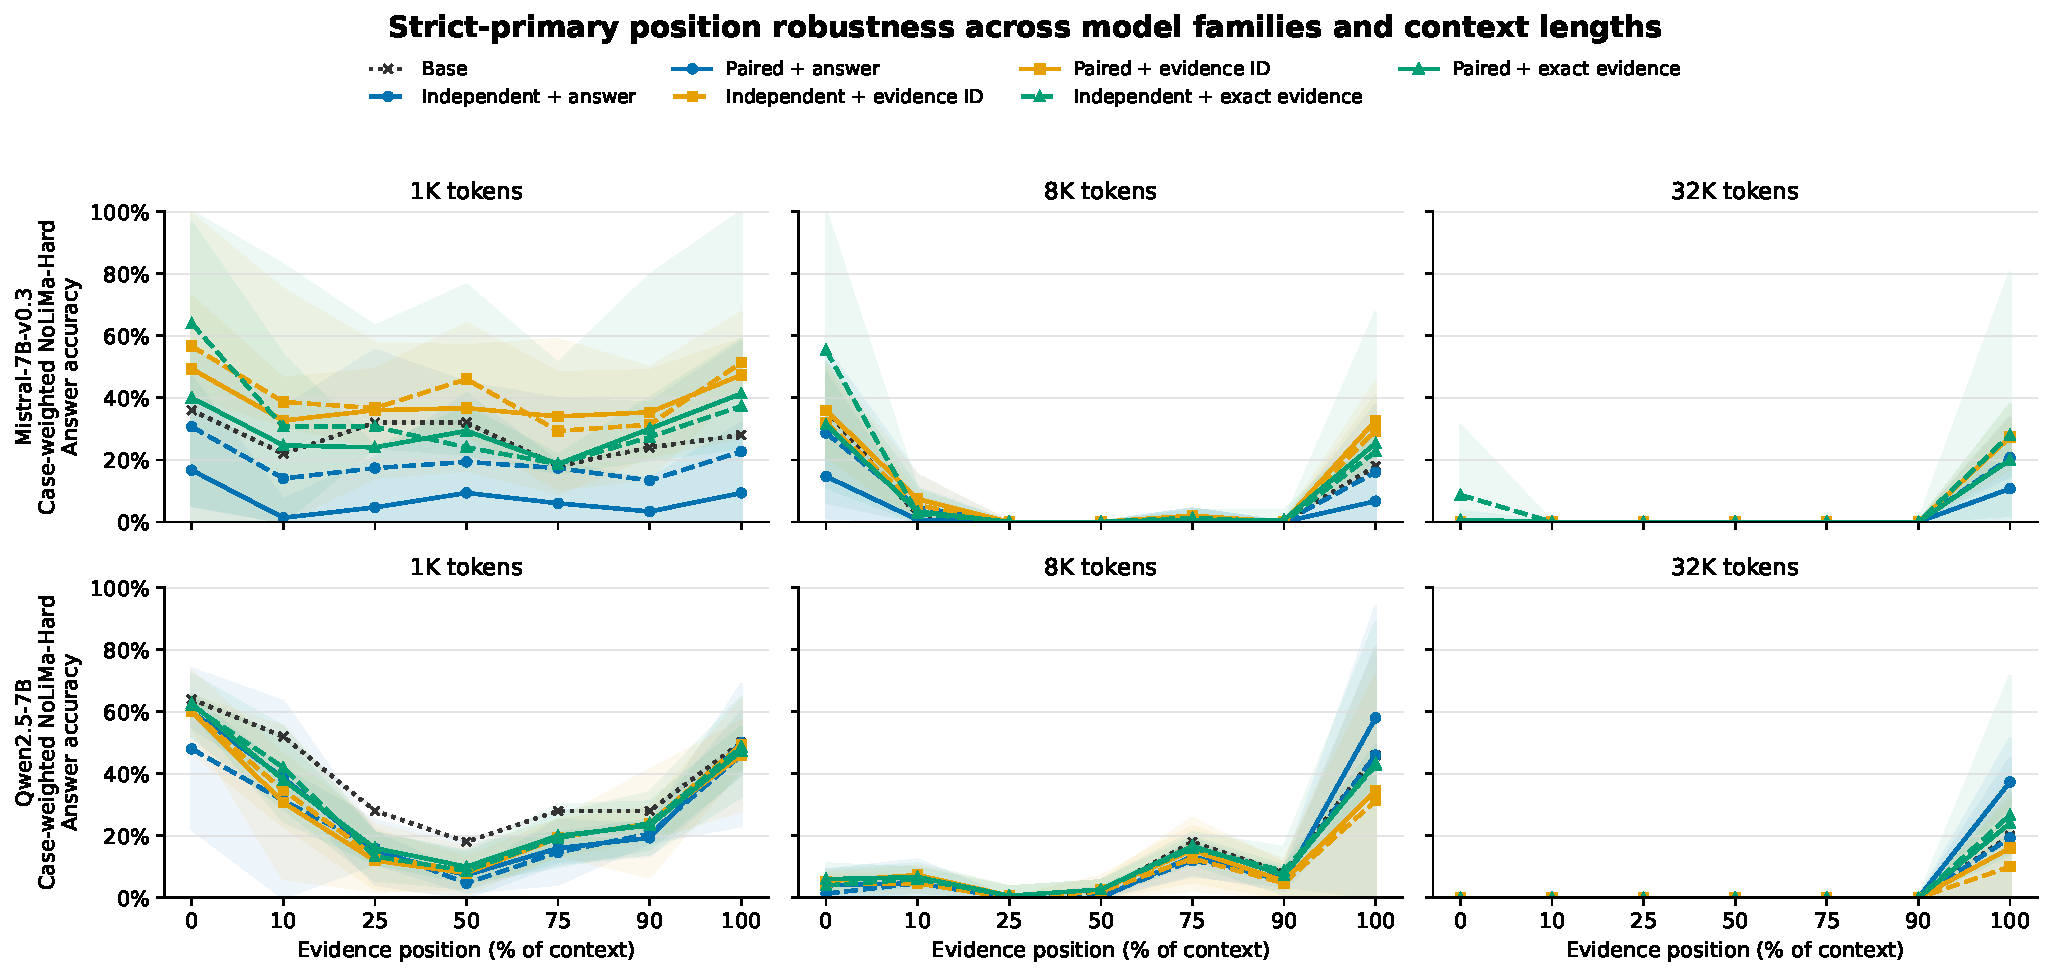
\includegraphics[width=\textwidth]{figures/factorial_position_curves.pdf}%
}{\fbox{\parbox{0.94\textwidth}{\centering\pending{copy audited factorial position figure}}}}
\caption{Primary strict block-complete NoLiMa-Hard answer accuracy across seven evidence positions, case-weighted over the 2/6/2 underlying semantic cases in the three task strata. Rows denote model family and columns context length. Color denotes supervision and solid versus dashed lines denote paired versus independent construction. Bands are 95\% Student-$t$ intervals over independently trained seeds, clipped only for display; the fixed Base has no seed interval and exact values are provided in the companion CSV.}
\label{fig:position}
\end{figure*}

\subsection{Natural multi-document transfer}

\pending{report HotpotQA, 2WikiMQA, MuSiQue, and pooled token-F1, including negative or null treatment effects}. Because LongBench does not annotate movable gold evidence here, these scores establish natural transfer only.

\begin{table*}[t]
\centering
\small
\caption{Primary strict block-complete LongBench multi-document QA token-F1. Treatment values average independently trained seeds and Base is fixed. Scores use the maximum official English QA F1 over references; the three tasks contain 200 questions each.}
\label{tab:longbench}
\begin{tabular}{lllrrrr}
\toprule
Model & Pairing & Supervision & HotpotQA & 2WikiMQA & MuSiQue & Pooled \\
\midrule
\GeneratedLongBenchRows
\bottomrule
\end{tabular}
\end{table*}

\begin{table*}[t]
\centering
\scriptsize
\setlength{\tabcolsep}{3pt}
\caption{Key strict block-complete factorial contrasts in percentage points, shown as seed-level mean [95\% Student-$t$ interval]. Positive $\Delta$Worst is better, whereas positive $\Delta$Gap is worse; positive LongBench $\Delta$F1 is better. These contrasts predate the realized-subset correction; complete per-seed contrasts, within-seed paired bootstrap intervals, and Holm-adjusted tests are included in the released analysis files.}
\label{tab:factorial-contrasts}
\begin{tabular}{llrrrrr}
\toprule
Model & Contrast & Rule $\Delta$Worst & Rule $\Delta$Gap & NoLiMa $\Delta$Worst & NoLiMa $\Delta$Gap & LongBench $\Delta$F1 \\
\midrule
\GeneratedFactorialContrastRows
\bottomrule
\end{tabular}
\end{table*}

\subsection{Mechanism and capability retention}

The exploratory Qwen representative separates three otherwise conflated failure modes. Oracle-short performance is near ceiling for Base and all four corner treatments, so answer generation from an isolated gold passage is not the dominant bottleneck. Exact-evidence treatments substantially improve locate-only quotation, but this gain does not carry over to free-answer accuracy or to oracle-long evidence use under distractors. Paired answer supervision is the only Qwen corner that materially improves oracle-long accuracy, yet its free-answer score still does not exceed Base, consistent with better use of already exposed evidence but unresolved localization. These representative-seed diagnostics are not multi-seed treatment estimates; Table~\ref{tab:mechanism} reports the clustered intervals and the final paper will compare whether the same decomposition appears in Mistral.

The Qwen MMLU reanalysis passes the frozen two-point noninferiority margin for every treatment after correctness is separated from JSON closure. IFEval shows no Holm-significant treatment difference, but none of its strict-prompt intervals establishes the same noninferiority guarantee. We therefore report no detected instruction-following difference while retaining the uncertainty, rather than treating a nonsignificant test as equivalence. A treatment is interpreted as improving retrieval only if locate-only gains accompany free-task gains and oracle answer generation remains stable. \pending{compare these representative checks with the audited Mistral replication}.

\begin{table*}[t]
\centering
\small
\caption{Representative-seed short-context regression checks. MMLU is full-test format-robust option accuracy and IFEval is official strict prompt accuracy. Noninferiority passes only when the paired 95\% interval for treatment minus Base lies entirely above the frozen $-2$ pp margin. JSON validity is audited separately and is not required for MMLU correctness.}
\label{tab:regression}
\begin{tabular}{lllrrrr}
\toprule
Model & Pairing & Supervision & MMLU & MMLU NI & IFEval & IFEval NI \\
\midrule
\GeneratedRegressionRows
\bottomrule
\end{tabular}
\end{table*}

\begin{table*}[t]
\centering
\small
\caption{Representative-seed NoLiMa mechanism decomposition. Locate-only requests the quote; oracle-long moves gold evidence to a tagged block after the same long distractor context; oracle-short removes distractors. Values are clustered over the 10 semantic cases.}
\label{tab:mechanism}
\begin{tabular}{lllrrrr}
\toprule
Model & Pairing & Supervision & Free answer & Locate quote & Oracle long & Oracle short \\
\midrule
\GeneratedMechanismRows
\bottomrule
\end{tabular}
\end{table*}

\subsection{Descriptive failure taxonomy}

The two historical post-pilot fixed-100 Qwen NoLiMa catalogs agree on the qualitative failure shape. Answers change somewhere across the seven positions in roughly nine of ten eligible within-run groups, and edge-success/middle-failure groups are about four times as common as the reverse pattern. Invalid JSON and output-cap hits remain below one percent, so formatting failures cannot explain the low semantic answer accuracy. In matched Base--treatment comparisons, Base-only successes outnumber treatment-only successes in both seeds, consistent with the absence of a stable partial-dose treatment advantage. \pending{replace this diagnostic account with the strict Qwen and prospective Mistral pre-specified row-, group-, and Base--treatment failure rates, then discuss representative identifier-fingerprinted cases without reproducing benchmark text}. We keep the three denominator types separate and use these cases only to illustrate aggregate results, not to select a treatment or add post-hoc significance claims.

\section{Discussion}

The factorial design separates three conclusions that are often conflated. First, a flat in-distribution position curve can coexist with poor semantic or natural transfer. Second, answer-only correctness does not establish verifiable evidence use. Third, a balanced position histogram is not necessarily equivalent to showing the same underlying fact across positions. \pending{revise these interpretations against strict effects and model-family interaction}.

The experiment is designed to support informative negative results. If all six strict block-96 treatments converge on the same OOD score, the supported conclusion is that one-pass low-budget supervised repair is not sensitive to these factors at the available resolution. If rule accuracy improves but NoLiMa and LongBench do not, the conclusion is distribution-specific memorization or template adaptation rather than robust context utilization.

\section{Limitations}

The study uses two approximately 7B model families and cannot establish scaling laws. QLoRA may interact with model family and position encoding differently from full-parameter training. The strict callback stops at step 96 during the first 60-step warmup plus 36 subsequent steps of a 2,000-step cosine horizon; this is a low-budget, one-pass adapter regime rather than an optimized full-convergence recipe. Our attribution therefore concerns which factors help under that fixed regime, not whether longer or full-parameter training could remove the failure. The strict correction was designed only after Qwen NoLiMa and partial LongBench outputs existed. Its selection rule is deterministic, score-independent, and applied to all six cells and all three seeds, but the Qwen correction is still post hoc; only Mistral tests the corrected design prospectively. We retain the original fixed-100 artifacts and their failed realized-subset gate so that this limitation is independently auditable. The NoLiMa-Hard gate contains only 10 underlying semantic cases repeated over books, lengths, and placements; inference must respect that grouping and claims cannot treat 1,050 prompts as independent semantic questions. LongBench supplies natural contexts but no controlled evidence relocation or exact evidence labels in our selected tasks. Each model family's deterministic Base generations are reused across treatment seeds rather than presented as independent model-training replicates; seed-level treatment intervals therefore quantify adapter/data-seed variation around a fixed Base, not uncertainty over base-model pretraining or model selection. Consequently, seed-level intervals are necessarily wide and cross-family differences are treated as descriptive interactions rather than precise population estimates. Finally, exact quotation is a verifiability proxy, not a complete measure of faithful reasoning.

\section{Ethics, Licensing, and Reproducibility}

NoLiMa data are used for non-commercial research under the Adobe Research License and are distributed through source pointers and generation hashes rather than relicensed. The LongBench repository is MIT licensed, while constituent datasets retain their original terms. The synthetic data contain generated facts rather than personal information. Public failure catalogs use one-way fingerprints in place of benchmark text and raw identifiers. We release no model-service credentials, machine passwords, or private paths.

The full audited evidence tree retains every result row with its model condition, sample and position-equivalent group, target, raw generation, parsed JSON, applicable metrics, finish reason, and output-token count. The public release excludes raw benchmark and generation JSONL rather than silently relicensing benchmark text; it provides pinned reconstruction scripts and hashes, license-safe per-sample failure records, model revision and file hashes, data manifests, environment and GPU metadata, per-step training traces, all bootstrap indices, analysis CSV/JSON, and vector/raster figures with table alternatives and alt text.

All training and generation workloads are executed sequentially on one 32 GB RTX 5090-class instance rather than hidden behind multi-instance parallelism. \pending{insert the audited queue wall time, GPU-hours, and rental cost after the final evidence manifest closes}. We report measured hardware and wall time so that compute can be compared, but do not estimate carbon emissions because the cloud vendor does not disclose machine power attribution, data-center location, or PUE for this rental.

\section{Conclusion}

We presented a matched factorial framework for attributing long-context position robustness to explicit cross-position pairing and supervision granularity. \pending{insert final evidence-grounded conclusion after both model families, all seeds, OOD suites, and diagnostics pass audit}.

\appendix

\section{Frozen training configuration}

All strict primary cells use the same implementation and hyperparameters shown in Table~\ref{tab:training-config}. A run resumes only from its own latest checkpoint; an already audited step-96 checkpoint is never retrained. Model weights are loaded from local snapshots at pinned revisions, and pretokenized data must match the tokenizer and chat-template fingerprint before CUDA work begins. The historical step-100 artifacts are retained under separate roots and cannot satisfy the primary completion gate.

\begin{table}[h]
\centering
\small
\caption{Frozen QLoRA configuration for every strict primary treatment.}
\label{tab:training-config}
\begin{tabularx}{\linewidth}{@{}lX@{}}
\toprule
Item & Value \\
\midrule
Quantization & 4-bit NF4, double quantization, BF16 compute \\
LoRA & rank 16, $\alpha=32$, dropout 0.05, all linear layers \\
Objective & completion-only cross entropy, no packing \\
Maximum sequence length & 8,320 tokens \\
Batching & one sequence/device, accumulation 1 \\
Optimizer & paged AdamW 8-bit \\
Learning-rate schedule & peak $2\times10^{-4}$; cosine over a 2,000-step horizon \\
Warmup and stopping & 60-step warmup (3\% of horizon); callback at exactly step 96 \\
Precision/runtime & BF16, TF32, gradient checkpointing, SDPA \\
Seed IDs & 20260825, 20260826, 20260827; Qwen rerun is post-hoc corrective, Mistral prospective \\
\bottomrule
\end{tabularx}
\end{table}

\section{Evaluation and decoding inventory}

Table~\ref{tab:evaluation-config} records the frozen inference windows and decoding caps. Every rendered prompt plus its output cap must fit the listed window; the window value is not presented as the realized prompt length. All suites use greedy decoding (temperature 0) with a fixed runtime seed; batch size and vLLM engine settings are recorded per run and held constant within each suite. Controlled rule, NoLiMa, LongBench, and MMLU generations request schema-constrained JSON. For the first three suites, format validity is part of the structured-task diagnostics. For MMLU, correctness is rescored from the option letter independently of JSON closure while validity and truncation are reported separately. IFEval is deliberately unconstrained because the official instructions often require exact free-form formatting; its raw text is scored by the pinned official verifier.

\begin{table}[h]
\centering
\small
\caption{Evaluation inventory per model condition. Counts exclude bootstrap replicates.}
\label{tab:evaluation-config}
\begin{tabular}{lrrrl}
\toprule
Suite & Rows & Window & Max output & Primary unit \\
\midrule
Matched rule & 4,200 & 32,768 & 176 & position-equivalent group \\
NoLiMa-Hard & 1,050 & 32,768 & 176 & semantic case/group \\
LongBench QA & 600 & 32,768 & 96 & benchmark question \\
NoLiMa diagnostics & 1,350 & 32,768 & 176 & semantic case \\
MMLU & 14,042 & 2,048 & 32 & test question \\
IFEval & 541 & 4,096 & 1,024 & prompt/instruction \\
\bottomrule
\end{tabular}
\end{table}

\section{Artifact and claim audit}

The release distinguishes raw generations, within-seed paired bootstrap analyses, seed-level summaries, and paper-facing numbers. Raw outputs are resumable JSONL files with immutable data and adapter hashes. Each within-seed analysis saves its 5,000 resampling indices. Seed-level aggregation accepts exploratory, corrective, and confirmatory designations explicitly; exploratory runs are excluded from primary summaries, while each included model family must have at least two independently trained eligible seeds. Finally, the generated TeX table records SHA-256 values for all seed-level inputs; submission audit rejects unresolved placeholders, missing figures or citations, secrets, and absolute machine paths. Author metadata remains the only non-experimental item that cannot be finalized autonomously.

\bibliographystyle{plainnat}
\bibliography{references}

\end{document}
